\let\negmedspace\undefined
\let\negthickspace\undefined
\documentclass[journal]{IEEEtran}
\usepackage[a5paper, margin=10mm, onecolumn]{geometry}
%\usepackage{lmodern} % Ensure lmodern is loaded for pdflatex
\usepackage{tfrupee} % Include tfrupee package

\setlength{\headheight}{1cm} % Set the height of the header box
\setlength{\headsep}{0mm}     % Set the distance between the header box and the top of the text

\usepackage{gvv-book}
\usepackage{gvv}
\usepackage{cite}
\usepackage{amsmath,amssymb,amsfonts,amsthm}
\usepackage{algorithmic}
\usepackage{graphicx}
\usepackage{textcomp}
\usepackage{xcolor}
\usepackage{txfonts}
\usepackage{listings}
\usepackage{enumitem}
\usepackage{mathtools}
\usepackage{gensymb}
\usepackage{comment}
\usepackage[breaklinks=true]{hyperref}
\usepackage{tkz-euclide} 
\usepackage{listings}
% \usepackage{gvv}                                        
\def\inputGnumericTable{}                                 
\usepackage[latin1]{inputenc}                                
\usepackage{color}                                            
\usepackage{array}                                            
\usepackage{longtable}                                       
\usepackage{calc}                                             
\usepackage{multirow}                                         
\usepackage{hhline}                                           
\usepackage{ifthen}                                           
\usepackage{lscape}
\begin{document}

\bibliographystyle{IEEEtran}
\vspace{3cm}

\title{1.5.9}
\author{EE24BTECH11001 - Aditya Tripathy}
% \maketitle
% \newpage
% \bigskip
{\let\newpage\relax\maketitle}

\renewcommand{\thefigure}{\theenumi}
\renewcommand{\thetable}{\theenumi}
\setlength{\intextsep}{10pt} % Space between text and floats


\numberwithin{equation}{enumi}
\numberwithin{figure}{enumi}
\renewcommand{\thetable}{\theenumi}


\textbf{Question}:\\
In what ratio does the $x$-axis divide the line segment joing the points $\vec{A} \brak{3,6}$ and $\vec{B}\brak{-12,-3}$?
\\
\textbf{Solution: }\\
From \brak{1.1.4.1}, if $\vec{D}$ divides $\vec{BC}$ in the ratio $k:1$,

\begin{align}
	\vec{D} = \frac{k\vec{C} + \vec{B}}{k+1}
\end{align}
 \\
Since the point lies on the $x$-axis, it is of the form $\brak{x,0}$. So, 

\begin{align}
	\myvec{x \\ 0} = \frac{\myvec{-12\\-3} + \myvec{3\\6}}{k+1}\\
	\myvec{x\\0} = \frac{\myvec{-12k+3\\ \\-3k+6}}{k+1}\\
	\myvec{x\\0} = \myvec{\frac{-12k+3}{k+1}\\ \\ \frac{-3k+6}{k+1}}\\
\end{align}
On comparing the entries in the two vectors we get, 
\begin{align}
	0 = \frac{-3k+6}{k+1} \implies k = 2\\
	x = \frac{-12k+3}{k+1} \implies x = -7\\
\end{align}
Hence the $x$-axis divides the line segment joining $\vec{A}$ ,$\vec{B}$ in the ratio $2:1$
\begin{figure}[h!]
   \centering
   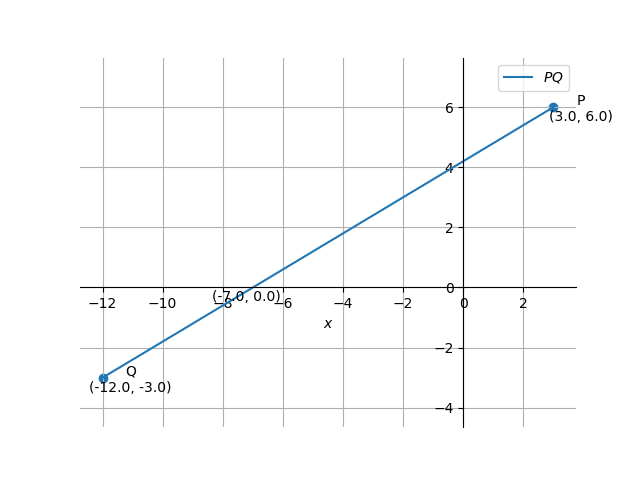
\includegraphics[width=0.7\linewidth]{figs/fig.png}
   \caption{Point joining A and B}
   \label{stemplot}
\end{figure}
\end{document}  
\end{document}

